\chapter{Basics}
\label{chapter:basics}

\section{Loudness}

Including the human perception in the algorithm is a complex task as for example absolute threshold of hearing and the subjective perception of sound pressure are varying for different frequencies (see \ref{LDNSGraph}).\\

\begin{figure}[H]
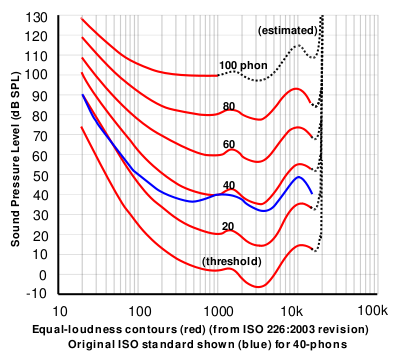
\includegraphics[width=0.5\textwidth]{images/loudnessGraph}
	\centering
	\caption{Loudness perception\cite{wikiLoud}}
	\label{LDNSGraph}
\end{figure}

While gathering information on how to improve the plug-in in terms of human perception the ITU-R BS.1770-4\cite{ITUalgo} algorithm was evaluated. This algorithm classifies an audio file for its humanly perceived loudness. It is mainly used by television and music streaming services as the program loudness can be kept steady while switching content. As the human perception is of substantial interest for mixing a song, this was interesting for this study. Due to a good documentation about how to implement the loudness algorithm a copy of it was build in Python and it was decided which elements to be adopted in the plug-in. The first and second element were two filters. Their use is to mimic the human perception of sound pressure at different frequencies. The first filter is a low cut for the reason that human hearing is insensitive to low frequencies. The second filter is a high shelf and is ‘\textit{used to account for the acoustic effects of the head}’\cite{ITUalgo}. This imitation of the human hearing is substantially simplified but cost-effective in terms of computation. The low cut filter has a cutoff frequency of 38 Hz, the high shelf of around 1681 Hz.\\

\begin{figure}[H]
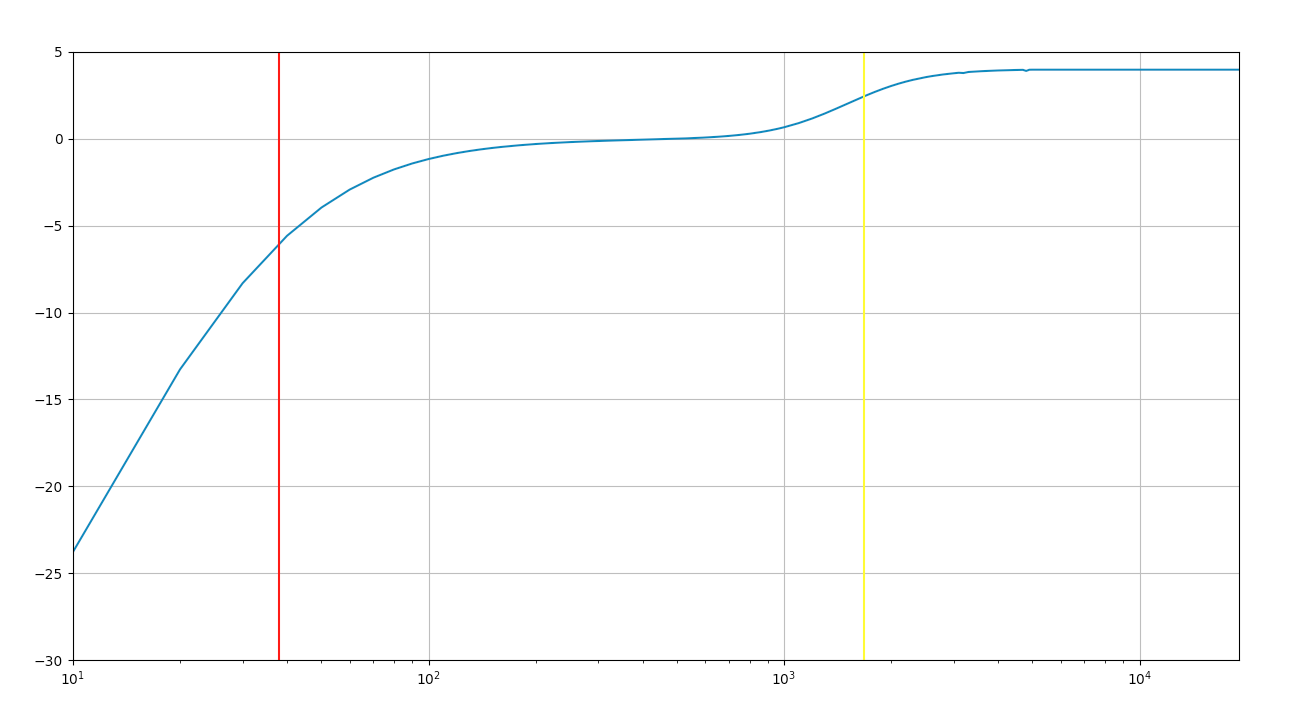
\includegraphics[width=0.8\textwidth]{images/filter_test}
	\centering
	\caption{Plotted outcome of adopted filter implementation for the audible spectrum of frequencies}
	\label{filterTest}
\end{figure}

The filter section is followed by the determination of a root mean square (RMS) value for time windows of 400ms overlaping 75\% (a value is saved every 100ms). This means it is calculating the root of the average from the squares of each sample in the set time window which equals the power of the signal.\\
RMS calculation is used because it is part of the imitation of human perception: a human will not interpret a small impulse of a handful of samples as loud as a audio signal at the same level of longer duration.  For example ‘\textit{a 3-msec pulse must have a level about 15 dB higher to sound as loud as a 0.5-sec (500-msec) pulse}'\cite{masterHA}.\\
Subsequently all rms values below a absolute threshold of -70LKFS\footnote{definition in \cite{ITUalgo}} are sorted out by a gate and a average value is determined. Another gate of -10LU below the average is applied on the rms values and a second averaging of measurements is performed. The resulting average is the loudness of the processed audio file.\\

\section{Vocal Rider}

The 'Vocal Rider' by Waves is a published audio plug-in which realizes a automatic gain adaption for vocal signals.

\begin{figure}[H]
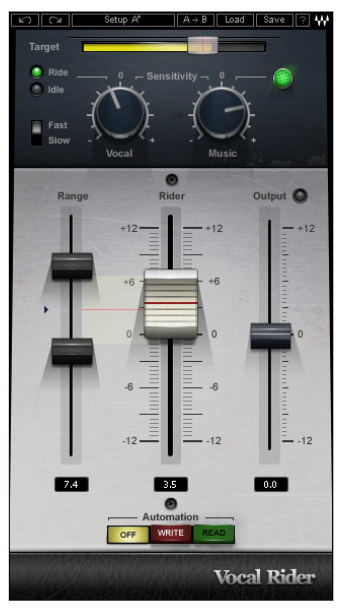
\includegraphics[width=0.35\textwidth]{images/vocalRiderUI}
	\centering
	\caption{UI of Waves 'Vocal Rider'\cite{vocalRiderM}}
	\label{VRUI}
\end{figure}

The vocal signal's level is adjusted to the set \textit{target} value (at top of Fig. \ref{VRUI}). The '\textit{target sets the reference range for vocal mix positioning. [It] (…) will move the Rider Fader’s ‘0’ calibration.}'\cite{vocalRiderM}. Additional a user can control the maximal gain adaption with the '\textit{range}' slider and adjust the resulting level to the backtrack via a output gain. For results depending on the instrumental backtrack a side chain input can be used and adjusted with the '\textit{music}' potentiometer.\\
As in this study the same basic idea is realized with a independent approach it is possible to adopt useful results from the comparison (see chapter \ref{chapter:comparison}) of both plug-ins and remain with potential advantages.\\

\section{Optimization}

For the comparison in chapter \ref{chapter:comparison} optimization methods were used to find parameters for the study plug-in to get to similar results as the 'Vocal Rider' does. Therefore the scipy\cite{scipy} methods scipy.optimize.brute and scipy.optimize.minimize were used.\\
Previously a function had to be written which returns the current problem as a number. Thereby a smaller number equals a smaller problem.\\
The '\textit{brute}' optimization algorithm '\textit{computes the function’s value at each point of a multidimensional grid of points, to find the global minimum of the function}'\cite{scipyB}. The according '\textit{grid}' is therefore previously defined for the current optimization problem. This is done by initializing a set of user defined bounds and step sizes for each of the parameters which a transferred to the function to be optimized.\\
The '\textit{minimize}' optimization algorithm per default '\textit{uses the L-BFGS-B algorithm ... for bound constrained minimization}'\cite{scipyM}. This algorithm is able to compute faster and more selective but needs a good inital parameter guess to get to a proper result.\\

